\documentclass[12pt,a4paper]{article}
\usepackage[utf8]{inputenc}
\usepackage[T1]{fontenc}
\usepackage{amsmath,amssymb,amsthm,mathtools}
\usepackage{hyperref}
\usepackage{cleveref}
\usepackage{graphicx}
\usepackage{geometry}
\usepackage{tikz-cd}
\usepackage{tikz}
\usetikzlibrary{decorations.pathmorphing,arrows.meta,positioning,calc}
\usepackage{enumitem}
\usepackage{xcolor}
\usepackage{fancyhdr}
\usepackage{everypage}
\usepackage{abstract}
\usepackage{setspace}
\usepackage{booktabs}
\usepackage{float}
\usepackage{caption}
\usepackage{listings}
\geometry{margin=1in}

\definecolor{grokgray}{RGB}{110,110,110}
\AddEverypageHook{%
  \ifnum\value{page}=1
    \begin{tikzpicture}[remember picture, overlay]
      \node[rotate=90, anchor=south, font=\Large\sffamily\bfseries\color{grokgray}, inner sep=0pt]
      at ([xshift=38pt, yshift=0.52\paperheight]current page.south west)
      {GrokRxiv:2026.03.structural-dna-memory-layout\quad [\,bio.PL\,]\quad 31 Mar 2026};
    \end{tikzpicture}
  \fi
}

\theoremstyle{plain}
\newtheorem{theorem}{Theorem}[section]
\newtheorem{proposition}[theorem]{Proposition}
\newtheorem{lemma}[theorem]{Lemma}
\newtheorem{corollary}[theorem]{Corollary}
\theoremstyle{definition}
\newtheorem{definition}[theorem]{Definition}
\newtheorem{example}[theorem]{Example}
\newtheorem{remark}[theorem]{Remark}

% Listings configuration
\lstset{
  basicstyle=\small\ttfamily,
  keywordstyle=\color{blue!70!black}\bfseries,
  commentstyle=\color{green!50!black}\itshape,
  stringstyle=\color{red!60!black},
  numbers=left,
  numberstyle=\tiny\color{gray},
  numbersep=5pt,
  breaklines=true,
  frame=single,
  rulecolor=\color{gray!30},
  backgroundcolor=\color{gray!5},
  captionpos=b,
  tabsize=2,
  showstringspaces=false
}

\lstdefinelanguage{DNALang}{
  keywords={type, data, class, instance, where, let, in, do, if, then, else, case, of, module, import, deriving, newtype, forall},
  morekeywords={Linear, Telomere, Centromere, TAD, ChromatinLoop, Structure, GenomeLayout, Territory, Compartment, LAD, Resource, Consume, Regenerate, Barrier, Mutex, Pointer, Deref, MemoryBank},
  sensitive=true,
  morecomment=[l]{--},
  morecomment=[s]{\{-}{-\}},
  morestring=[b]",
}

\title{\textbf{Structural DNA as Memory Architecture:\\A Type-Theoretic Framework for Genome Organization}}
\author{
  Matthew Long\\
  \textit{The YonedaAI Collaboration}\\
  Chicago, IL\\
  \texttt{matt@yoneda.ai}
}
\date{March 31, 2026}

\begin{document}
\maketitle

\begin{abstract}
We present a type-theoretic framework that formalizes the structural elements of the genome---telomeres, centromeres, topologically associating domains (TADs), chromatin loops, and nuclear compartments---as components of a memory architecture in a programming language. Telomeres are modeled as linear resources with a bounded consumption budget, where each cell division consumes one unit and telomerase provides controlled regeneration. Centromeres are cast as synchronization primitives that enforce barriers and mutual exclusion during mitotic chromosome segregation. Topologically associating domains become memory segments with boundary-enforced encapsulation via CTCF and cohesin. Chromatin loops are formalized as typed pointers implementing enhancer-promoter communication through controlled dereferencing, while nuclear organization---chromosome territories, A/B compartments, and lamina-associated domains---maps onto a multi-level memory hierarchy. We prove three central theorems: the Telomere Linear Type Theorem establishing resource soundness, the TAD Encapsulation Theorem guaranteeing segment isolation, and the Territory Memory Protection Theorem ensuring inter-chromosomal access control. A Haskell implementation demonstrates the executable semantics of the framework. This work provides a rigorous computational lens through which genome organization can be analyzed, offering new perspectives on aging, cancer, and developmental gene regulation.
\end{abstract}

\tableofcontents
\newpage

%% ============================================================
%%  SECTION 1: INTRODUCTION
%% ============================================================
\section{Introduction}\label{sec:intro}

The genome is not merely a linear sequence of nucleotides encoding proteins. It is a three-dimensional, dynamically regulated structure whose spatial organization is integral to its function. Over the past two decades, advances in chromosome conformation capture (3C, 4C, Hi-C) and super-resolution microscopy have revealed that the genome possesses a rich hierarchical architecture: chromosomes occupy distinct territories within the nucleus, fold into compartments and topologically associating domains, and form specific long-range contacts through chromatin looping \cite{lieberman2009comprehensive, dixon2012topological, rao20143d}. These structural features are not epiphenomenal---they actively regulate gene expression, DNA replication, and repair.

From a computational perspective, this architecture bears a striking resemblance to the memory systems of modern computers. Just as a computer organizes memory into hierarchical levels (registers, cache, RAM, disk) with access control, segmentation, and pointer-based indirection, the genome organizes its information into territories, compartments, domains, and loops with boundary-enforced isolation, accessibility gradients, and specific long-range contacts that function as pointers. This analogy is not merely metaphorical: we argue that it can be made precise using the tools of type theory and programming language semantics.

\subsection{Motivation: Beyond Sequence}

Classical molecular biology adopted a largely one-dimensional view of the genome. The Central Dogma---DNA $\to$ RNA $\to$ Protein---treats the genome as a tape to be read, and regulatory elements as annotations on that tape. However, this view cannot account for several fundamental observations:

\begin{enumerate}[label=(\roman*)]
  \item \textbf{Enhancer-promoter specificity.} Enhancers can activate promoters hundreds of kilobases away while skipping over intervening genes. The mechanism is three-dimensional looping, not linear scanning.
  \item \textbf{Position effects.} Identical transgenes inserted at different genomic locations exhibit dramatically different expression levels, depending on the local chromatin environment and nuclear position.
  \item \textbf{Replication timing.} The genome is replicated in a stereotyped temporal order that correlates with its spatial compartmentalization, not its linear position.
  \item \textbf{Aging and telomere attrition.} The progressive shortening of telomeres with each cell division imposes a hard limit on replicative lifespan---a phenomenon that has no purely sequence-level explanation but is naturally captured by linear resource types.
\end{enumerate}

These observations demand a framework that treats genome \emph{structure} as a first-class computational concept. Programming language theory provides exactly such tools.

\subsection{Type Theory as a Lens}

Type theory, originally developed for the foundations of mathematics and the design of programming languages, provides a rigorous framework for reasoning about resources, access control, and composition. In particular:

\begin{itemize}
  \item \textbf{Linear types} \cite{girard1987linear, wadler1990linear} model resources that must be used exactly once, capturing the irreversible consumption of telomeric repeats during DNA replication.
  \item \textbf{Synchronization primitives}---mutexes, barriers, and semaphores---formalize the coordination required during mitosis, where the spindle assembly checkpoint ensures that all chromosomes are properly attached before anaphase proceeds.
  \item \textbf{Memory segmentation} and \textbf{capability-based access control} model the insulation properties of TAD boundaries, which restrict regulatory interactions to within-domain contacts.
  \item \textbf{Pointer types} with controlled dereferencing capture the semantics of chromatin loops, where a specific genomic locus (the enhancer) ``points to'' a distant locus (the promoter) and activates it through physical contact.
\end{itemize}

The contribution of this paper is to systematize these analogies into a coherent type-theoretic framework, prove formal properties of the resulting system, and provide an executable implementation in Haskell.

\subsection{Related Work}

The analogy between biological systems and computation has a long history, from von Neumann's self-reproducing automata to Bray's computational model of cellular signaling \cite{bray1995protein}. More recently, Regev and Shapiro modeled biological processes using the $\pi$-calculus \cite{regev2001representation}, and Cardelli developed process algebras for molecular biology \cite{cardelli2005abstract}. In the genomics domain, the ENCODE project systematically annotated functional elements \cite{encode2012integrated}, and subsequent work on 3D genome organization \cite{dekker2013exploring} has revealed the structural features we formalize here.

Our work differs from these approaches in two key respects. First, we focus specifically on \emph{structural} DNA elements---the architectural components of the genome rather than the coding or regulatory sequences. Second, we use \emph{type theory} rather than process algebra, which allows us to reason about resource consumption, access control, and memory layout in a unified framework.

\subsection{Overview}

The remainder of this paper is organized as follows. \Cref{sec:telomeres} formalizes telomeres as linear resources. \Cref{sec:centromeres} models centromeres as synchronization primitives. \Cref{sec:tads} treats TADs as memory segments. \Cref{sec:structure-type} introduces the formal \texttt{Structure} type. \Cref{sec:loops} models chromatin loops as pointers. \Cref{sec:nuclear} maps nuclear organization onto a memory hierarchy. \Cref{sec:formal} presents our main theorems with proofs. \Cref{sec:haskell} provides an executable Haskell implementation. \Cref{sec:discussion} discusses implications and future directions.


%% ============================================================
%%  SECTION 2: TELOMERES AS LINEAR RESOURCES
%% ============================================================
\section{Telomeres as Linear Resources}\label{sec:telomeres}

\subsection{Biological Background}

Telomeres are repetitive nucleoprotein structures at the ends of linear chromosomes, consisting of tandem repeats of the hexanucleotide sequence TTAGGG in vertebrates. In humans, telomeres are approximately 10--15 kilobases long at birth and shorten by 50--200 base pairs with each round of DNA replication, due to the end-replication problem: the lagging strand synthesis machinery cannot fully replicate the 3' end of a linear template \cite{blackburn2001telomere, olovnikov1973theory}.

This progressive shortening imposes a hard limit on the number of times a cell can divide. When telomeres reach a critically short length, the cell enters replicative senescence---a state of irreversible growth arrest first observed by Hayflick and Moorhead \cite{hayflick1961serial}. The Hayflick limit, typically 40--60 divisions for human fibroblasts, is thus directly determined by the initial telomere length and the rate of per-division attrition.

The enzyme telomerase, a reverse transcriptase that extends telomeric repeats, is active in germ cells, stem cells, and most cancer cells, but is repressed in normal somatic cells. This creates a fundamental asymmetry: most cells have a finite replicative budget, while a privileged subset can regenerate their telomeric resources.

\subsection{Linear Types and Resource Consumption}

In linear type theory, a value of linear type must be used exactly once: it cannot be duplicated (no contraction) and cannot be discarded (no weakening). This precisely captures the biology of telomeric repeats: each repeat is consumed exactly once per cell division, and lost repeats cannot be recovered (in the absence of telomerase).

\begin{definition}[Telomere Type]\label{def:telomere-type}
A \emph{telomere} is a linear resource type parameterized by a natural number $n \in \mathbb{N}$ representing the number of remaining repeats:
\[
  \texttt{Telomere}(n) : \texttt{LinearType}
\]
The \emph{division} operation consumes one unit of telomeric resource:
\[
  \texttt{divide} : \texttt{Telomere}(n+1) \multimap \texttt{Telomere}(n) \otimes \texttt{DaughterCell}
\]
where $\multimap$ denotes linear function and $\otimes$ denotes linear tensor (both outputs must be used).
\end{definition}

The key observation is that division is only well-typed when $n \geq 1$, i.e., when there is at least one telomeric repeat remaining. When $n = 0$, the type $\texttt{Telomere}(0)$ admits no further division:

\begin{definition}[Senescence]\label{def:senescence}
A cell with telomere state $\texttt{Telomere}(0)$ is \emph{senescent}. The only well-typed operation on a senescent telomere is:
\[
  \texttt{senesce} : \texttt{Telomere}(0) \multimap \texttt{SenescentCell}
\]
\end{definition}

This models the Hayflick limit as a type-level constraint: the type system \emph{statically} prevents division beyond the replicative capacity encoded in the telomere length.

\subsection{The Division Judgment}

We formalize the division process as a typing judgment in a linear type system. Let $\Gamma$ be a linear context (where each variable appears at most once):

\[
\frac{\Gamma \vdash t : \texttt{Telomere}(n+1)}{\Gamma \vdash \texttt{divide}(t) : \texttt{Telomere}(n) \otimes \texttt{DaughterCell}}
\quad (\textsc{T-Divide})
\]

\[
\frac{\Gamma \vdash t : \texttt{Telomere}(0)}{\Gamma \vdash \texttt{senesce}(t) : \texttt{SenescentCell}}
\quad (\textsc{T-Senesce})
\]

The linear context ensures that each telomere value is used exactly once. After division, the original telomere is consumed and replaced by a shorter one; there is no way to ``clone'' the original telomere without violating linearity.

\subsection{Telomerase as Resource Regeneration}

Telomerase provides a controlled mechanism for extending telomeric repeats. In our type system, telomerase is modeled as a special operation that is only available in certain cellular contexts (germ cells, stem cells):

\begin{definition}[Telomerase]\label{def:telomerase}
The telomerase operation regenerates telomeric resources:
\[
  \texttt{extend} : \texttt{Telomere}(n) \otimes \texttt{TelomeraseAccess} \multimap \texttt{Telomere}(n+k)
\]
where $k$ is the number of repeats added per extension cycle, and $\texttt{TelomeraseAccess}$ is a capability token that is available only in privileged cellular contexts.
\end{definition}

The capability token $\texttt{TelomeraseAccess}$ ensures that telomere extension cannot occur in arbitrary cells. This models the biological reality that telomerase is repressed in most somatic cells:

\[
\frac{\Gamma \vdash t : \texttt{Telomere}(n) \quad \Delta \vdash a : \texttt{TelomeraseAccess}}{\Gamma, \Delta \vdash \texttt{extend}(t, a) : \texttt{Telomere}(n+k)}
\quad (\textsc{T-Extend})
\]

\subsection{Cancer as Type Violation}

Cancer cells frequently reactivate telomerase, effectively obtaining unauthorized $\texttt{TelomeraseAccess}$ tokens. In our framework, this corresponds to a \emph{type violation}---a breach of the capability system that allows unlimited resource regeneration:

\begin{remark}[Oncogenic Telomerase Activation]
The activation of telomerase in somatic cells via TERT promoter mutations can be modeled as an unauthorized acquisition of $\texttt{TelomeraseAccess}$:
\[
  \texttt{mutate\_TERT} : \texttt{SomaticContext} \to \texttt{TelomeraseAccess} \quad \text{(UNSAFE)}
\]
This operation is marked \texttt{UNSAFE} because it bypasses the capability system, analogous to an unsafe cast in systems programming languages. The result is unbounded replicative potential---a hallmark of cancer.
\end{remark}

\subsection{Commutative Diagram: Telomere Lifecycle}

The following commutative diagram captures the lifecycle of a telomere through successive divisions and optional regeneration:

\begin{center}
\begin{tikzcd}[column sep=large, row sep=large]
  \texttt{Telomere}(n) \arrow[r, "\texttt{divide}"] \arrow[d, "\texttt{extend}"', dashed] & \texttt{Telomere}(n{-}1) \otimes \texttt{Daughter} \arrow[d, "\pi_1"] \\
  \texttt{Telomere}(n{+}k) \arrow[r, "\texttt{divide}"] & \texttt{Telomere}(n{+}k{-}1) \otimes \texttt{Daughter}
\end{tikzcd}
\end{center}

The dashed arrow indicates that extension requires a $\texttt{TelomeraseAccess}$ capability and is not available in all contexts. When the diagram commutes, it expresses the fact that extension followed by division yields a telomere whose length is $(n+k-1)$, which is strictly greater than the $(n-1)$ obtained by division alone. This captures the biological advantage of telomerase-positive cells.


%% ============================================================
%%  SECTION 3: CENTROMERES AS SYNCHRONIZATION PRIMITIVES
%% ============================================================
\section{Centromeres as Synchronization Primitives}\label{sec:centromeres}

\subsection{Biological Background}

The centromere is a specialized chromosomal region that serves as the attachment point for the mitotic spindle during cell division. In humans, centromeres are defined by the presence of alpha-satellite (alphoid) DNA repeats and the centromere-specific histone variant CENP-A. During mitosis, the centromere recruits a large protein complex called the kinetochore, which mediates attachment to spindle microtubules.

The spindle assembly checkpoint (SAC) is a surveillance mechanism that monitors kinetochore-microtubule attachments and delays anaphase onset until all chromosomes are properly bi-oriented on the spindle. The SAC effectively acts as a \emph{barrier synchronization}: the cell cannot proceed to chromosome segregation until every centromere reports proper attachment.

\subsection{The Barrier Model}

\begin{definition}[Centromere as Barrier]\label{def:centromere-barrier}
A \emph{centromere barrier} is a synchronization primitive for $2n$ chromosomes (where $n$ is the ploidy):
\[
  \texttt{Centromere} : \texttt{Barrier}(2n)
\]
The barrier requires $2n$ attachment signals before releasing:
\[
  \texttt{attach} : \texttt{Centromere}_i \otimes \texttt{Spindle}_j \multimap \texttt{Attached}(i, j)
\]
\[
  \texttt{checkpoint} : \bigotimes_{i=1}^{2n} \texttt{Attached}(i, j_i) \multimap \texttt{AnaphaseLicense}
\]
\end{definition}

The $\texttt{checkpoint}$ operation requires that \emph{all} $2n$ chromosomes have reported attachment. This is the barrier property: no thread (chromosome) can proceed past the barrier until all threads have arrived.

\subsection{Mutex for Kinetochore Assembly}

Each centromere must assemble exactly one kinetochore. Simultaneous assembly of multiple kinetochores on a single centromere (dicentric chromosomes) leads to catastrophic segregation errors. We model this as a mutual exclusion constraint:

\begin{definition}[Kinetochore Mutex]\label{def:kinetochore-mutex}
Each centromere provides a mutex for kinetochore assembly:
\[
  \texttt{Mutex}(\texttt{KinetochoreSlot}_i) : \texttt{MutexType}
\]
The operations are:
\begin{align*}
  \texttt{acquire} &: \texttt{Mutex}(\texttt{KinetochoreSlot}_i) \multimap \texttt{KinetochoreLock}_i \\
  \texttt{assemble} &: \texttt{KinetochoreLock}_i \multimap \texttt{Kinetochore}_i \otimes \texttt{Mutex}(\texttt{KinetochoreSlot}_i) \\
\end{align*}
The lock ensures that at most one kinetochore can be assembled per centromere at any time.
\end{definition}

\subsection{The Mitotic Synchronization Protocol}

Combining barriers and mutexes, the full mitotic synchronization protocol is:

\begin{enumerate}[label=\textbf{Step \arabic*:}]
  \item Each centromere $i$ acquires its kinetochore mutex and assembles a kinetochore.
  \item Each kinetochore attaches to a spindle fiber, producing an $\texttt{Attached}(i, j_i)$ token.
  \item The checkpoint barrier collects all $2n$ attachment tokens.
  \item Upon barrier release, an $\texttt{AnaphaseLicense}$ is produced, permitting chromosome segregation.
\end{enumerate}

The following diagram illustrates the synchronization flow:

\begin{center}
\begin{tikzcd}[column sep=small, row sep=large]
  \texttt{Cen}_1 \arrow[r, "\texttt{asm}"] \arrow[drr, phantom, "\cdots" description] & \texttt{Kin}_1 \arrow[r, "\texttt{att}"] & \texttt{Attached}(1,j_1) \arrow[dr] & \\
  \texttt{Cen}_i \arrow[r, "\texttt{asm}"] & \texttt{Kin}_i \arrow[r, "\texttt{att}"] & \texttt{Attached}(i,j_i) \arrow[r] & \texttt{License} \\
  \texttt{Cen}_{2n} \arrow[r, "\texttt{asm}"] \arrow[urr, phantom, "\cdots" description] & \texttt{Kin}_{2n} \arrow[r, "\texttt{att}"] & \texttt{Attached}(2n,j_{2n}) \arrow[ur] &
\end{tikzcd}
\end{center}

\begin{remark}[Checkpoint Failure and Aneuploidy]
If the SAC is compromised (e.g., by mutation of MAD2 or BUB1), the barrier can release prematurely. In our type system, this corresponds to weakening the barrier requirement---allowing $\texttt{AnaphaseLicense}$ to be produced with fewer than $2n$ attachment tokens. The result is aneuploidy (incorrect chromosome number), a hallmark of cancer cells.
\end{remark}


%% ============================================================
%%  SECTION 4: TADs AS MEMORY SEGMENTS
%% ============================================================
\section{Topologically Associating Domains as Memory Segments}\label{sec:tads}

\subsection{Biological Background}

Topologically associating domains (TADs) are megabase-scale regions of the genome within which chromatin interactions are significantly enriched relative to inter-domain interactions \cite{dixon2012topological, nora2012spatial}. TADs are demarcated by boundary elements, typically occupied by the insulator protein CTCF and the cohesin complex. These boundaries function as insulators that restrict the influence of enhancers and silencers to their containing domain.

Key properties of TADs include:
\begin{itemize}
  \item \textbf{Self-association}: Loci within a TAD interact with each other more frequently than with loci in adjacent TADs.
  \item \textbf{Boundary insulation}: TAD boundaries block the spread of regulatory signals. The insulation score at a boundary quantifies the reduction in cross-boundary contacts.
  \item \textbf{Conservation}: TAD boundaries are largely conserved across cell types and even across species, suggesting they are a fundamental unit of genome organization.
  \item \textbf{Hierarchical nesting}: TADs can contain sub-TADs, forming a hierarchical structure analogous to nested memory segments.
\end{itemize}

\subsection{TADs as Address Space Partitions}

We formalize TADs as segments of a genomic address space, where each segment has defined boundaries and access restrictions.

\begin{definition}[Genomic Address Space]\label{def:address-space}
The \emph{genomic address space} for a chromosome $c$ is a linearly ordered set:
\[
  \mathcal{A}_c = \{0, 1, \ldots, L_c - 1\}
\]
where $L_c$ is the length of chromosome $c$ in base pairs. A \emph{TAD} is a contiguous segment $[a, b) \subseteq \mathcal{A}_c$ together with boundary annotations:
\[
  \texttt{TAD}(a, b, \beta_L, \beta_R) : \texttt{MemorySegment}
\]
where $\beta_L, \beta_R : \texttt{Boundary}$ describe the left and right boundary elements.
\end{definition}

\begin{definition}[Boundary Type]\label{def:boundary}
A \emph{boundary} $\beta$ is characterized by:
\[
  \texttt{Boundary} = \left\{
    \begin{array}{l}
      \texttt{ctcf\_orientation} : \{\texttt{Forward}, \texttt{Reverse}\} \\
      \texttt{cohesin\_loaded} : \texttt{Bool} \\
      \texttt{insulation\_score} : [0, 1] \\
    \end{array}
  \right\}
\]
The insulation score $s \in [0,1]$ quantifies boundary strength: $s = 1$ indicates perfect insulation (no cross-boundary contacts), while $s = 0$ indicates no insulation.
\end{definition}

\subsection{CTCF and Cohesin as Boundary Enforcement}

The CTCF protein binds to specific DNA motifs in a strand-oriented manner. Convergently oriented CTCF sites (one forward, one reverse) form a TAD boundary by stalling the cohesin complex during loop extrusion:

\begin{definition}[Convergent CTCF Rule]\label{def:ctcf-convergent}
A valid TAD boundary requires convergent CTCF orientation:
\[
\frac{\beta_L.\texttt{ctcf\_orientation} = \texttt{Forward} \quad \beta_R.\texttt{ctcf\_orientation} = \texttt{Reverse}}{\texttt{TAD}(a, b, \beta_L, \beta_R) \text{ is well-formed}}
\quad (\textsc{TAD-Form})
\]
\end{definition}

This rule captures the biological observation that CTCF-mediated boundaries require convergent motif orientation. Disruption of a CTCF site (e.g., by mutation or methylation) weakens the boundary, allowing regulatory signals to leak across domains.

\subsection{Insulation as Access Control}

The insulation property of TAD boundaries is formalized as an access control mechanism. A regulatory element at address $x$ within TAD $T_1$ cannot access a target at address $y$ in a different TAD $T_2$ unless the intervening boundary is permeable:

\begin{definition}[TAD Access Control]\label{def:tad-access}
For loci $x \in \texttt{TAD}_1$ and $y \in \texttt{TAD}_2$ with $\texttt{TAD}_1 \neq \texttt{TAD}_2$, the access permission is:
\[
  \texttt{access}(x, y) = \prod_{b \in \texttt{Boundaries}(x,y)} (1 - b.\texttt{insulation\_score})
\]
Access is granted only when $\texttt{access}(x, y) > \theta$ for some threshold $\theta$. When all intervening boundaries have insulation score 1, the access product is 0 and no cross-domain interaction is possible.
\end{definition}

\subsection{Hierarchical TAD Nesting}

TADs form a hierarchical structure where sub-TADs are nested within larger TADs, analogous to nested memory segments or nested scoping in programming languages:

\begin{definition}[TAD Hierarchy]\label{def:tad-hierarchy}
A \emph{TAD hierarchy} on chromosome $c$ is a tree $\mathcal{T}$ where:
\begin{enumerate}[label=(\alph*)]
  \item Each node $v \in \mathcal{T}$ corresponds to a TAD $[a_v, b_v)$.
  \item If $v$ is a child of $u$, then $[a_v, b_v) \subseteq [a_u, b_u)$.
  \item Sibling TADs are non-overlapping: if $v_1, v_2$ are siblings, then $[a_{v_1}, b_{v_1}) \cap [a_{v_2}, b_{v_2}) = \emptyset$.
  \item The root spans the entire chromosome: $[a_{\text{root}}, b_{\text{root}}) = [0, L_c)$.
\end{enumerate}
\end{definition}

This hierarchy directly parallels the nesting of memory segments in a process's address space, where outer segments define coarse partitions and inner segments provide fine-grained access control.

\begin{center}
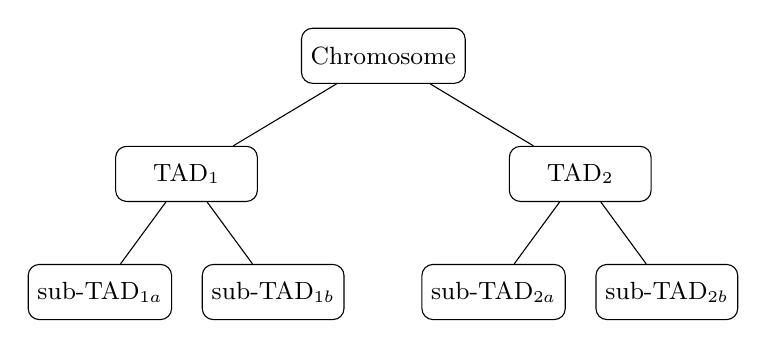
\begin{tikzpicture}[
  level distance=1.5cm,
  level 1/.style={sibling distance=5cm},
  level 2/.style={sibling distance=2.2cm},
  every node/.style={draw, rounded corners, minimum width=1.8cm, minimum height=0.7cm, align=center, font=\small}
]
\node {Chromosome}
  child {node {TAD$_1$}
    child {node {sub-TAD$_{1a}$}}
    child {node {sub-TAD$_{1b}$}}
  }
  child {node {TAD$_2$}
    child {node {sub-TAD$_{2a}$}}
    child {node {sub-TAD$_{2b}$}}
  };
\end{tikzpicture}
\end{center}

\subsection{Loop Extrusion and Segment Formation}

The formation of TADs is mechanistically linked to the process of loop extrusion by cohesin. Cohesin is loaded onto chromatin and processively extrudes a loop until it encounters a boundary element (typically a CTCF site). This process partitions the genome into segments in a manner analogous to a memory allocator partitioning an address space:

\begin{definition}[Loop Extrusion Partition]\label{def:loop-extrusion}
The loop extrusion process defines a partition $\mathcal{P}$ of the genomic address space:
\[
  \mathcal{P}(\mathcal{A}_c) = \{[a_1, b_1), [a_2, b_2), \ldots, [a_m, b_m)\}
\]
where each $[a_i, b_i)$ is a TAD, $b_i = a_{i+1}$ for all $i$ (complete partition), and each boundary $b_i$ coincides with a CTCF binding site. The partition is \emph{deterministic} given the positions and orientations of CTCF sites along the chromosome.
\end{definition}

This deterministic partitioning is analogous to a memory management unit (MMU) that divides physical memory into fixed segments based on hardware page boundaries. The CTCF sites serve as the ``page boundaries'' of the genome.


%% ============================================================
%%  SECTION 5: THE STRUCTURE TYPE
%% ============================================================
\section{The Structure Type}\label{sec:structure-type}

We now unify the preceding concepts into a single parametric type that captures the full structural state of a genome.

\subsection{Definition}

\begin{definition}[GenomeLayout]\label{def:genome-layout}
A \emph{genome layout} is a record type:
\[
  \texttt{GenomeLayout} = \left\{
    \begin{array}{ll}
      \texttt{chromosomes} &: \texttt{Vec}(\texttt{ChromosomeId}, 2n) \\
      \texttt{tad\_map} &: \texttt{ChromosomeId} \to \texttt{TADHierarchy} \\
      \texttt{loop\_set} &: \texttt{Set}(\texttt{ChromatinLoop}) \\
      \texttt{territories} &: \texttt{ChromosomeId} \to \texttt{NuclearRegion} \\
      \texttt{compartments} &: \texttt{GenomicLocus} \to \{\texttt{A}, \texttt{B}\} \\
    \end{array}
  \right\}
\]
\end{definition}

\begin{definition}[Structure Type]\label{def:structure-type}
The \emph{Structure} type is parameterized by a genome layout and includes topology, accessibility, and protection information:
\[
  \texttt{Structure}\langle G : \texttt{GenomeLayout} \rangle = \left\{
    \begin{array}{ll}
      \texttt{topology} &: \texttt{ContactMap}(G) \\
      \texttt{accessibility} &: \texttt{GenomicLocus} \to [0,1] \\
      \texttt{protection} &: \texttt{GenomicLocus} \to \texttt{ProtectionLevel} \\
      \texttt{telomeres} &: \texttt{ChromosomeId} \to \texttt{Telomere}(n_c) \\
      \texttt{centromeres} &: \texttt{ChromosomeId} \to \texttt{Centromere} \\
    \end{array}
  \right\}
\]
where:
\begin{itemize}
  \item $\texttt{ContactMap}(G)$ is a symmetric matrix $M$ with $M_{ij}$ representing the contact frequency between loci $i$ and $j$, consistent with the TAD structure in $G$.
  \item $\texttt{accessibility}(x)$ represents the chromatin openness at locus $x$, ranging from 0 (fully closed, heterochromatin) to 1 (fully open, active euchromatin).
  \item $\texttt{ProtectionLevel} \in \{\texttt{Open}, \texttt{Restricted}, \texttt{Protected}, \texttt{Silenced}\}$ is an access-control annotation.
\end{itemize}
\end{definition}

\subsection{Well-Formedness Conditions}

Not every assignment of fields constitutes a valid structure. We impose well-formedness conditions that capture the biological constraints:

\begin{definition}[Well-Formed Structure]\label{def:well-formed}
A structure $S : \texttt{Structure}\langle G \rangle$ is \emph{well-formed} if:
\begin{enumerate}[label=(WF\arabic*)]
  \item \textbf{TAD Consistency}: For all loci $x, y$ in the same TAD, $M_{xy} \geq \tau_{\text{intra}}$. For loci in different TADs separated by a strong boundary, $M_{xy} \leq \tau_{\text{inter}}$.
  \item \textbf{Compartment Coherence}: Loci in compartment A have $\texttt{accessibility}(x) \geq 0.5$, and loci in compartment B have $\texttt{accessibility}(x) < 0.5$.
  \item \textbf{Territory Exclusion}: For chromosomes $c_1 \neq c_2$, the nuclear regions $G.\texttt{territories}(c_1)$ and $G.\texttt{territories}(c_2)$ have bounded overlap.
  \item \textbf{Telomere Positivity}: For all chromosomes $c$, $S.\texttt{telomeres}(c) = \texttt{Telomere}(n_c)$ with $n_c \geq 0$.
\end{enumerate}
\end{definition}

\subsection{Morphisms of Structures}

Cellular processes that alter genome structure (differentiation, mitosis, DNA damage) can be modeled as morphisms between structure types:

\begin{definition}[Structure Morphism]\label{def:structure-morphism}
A \emph{structure morphism} $f : \texttt{Structure}\langle G_1 \rangle \to \texttt{Structure}\langle G_2 \rangle$ consists of:
\begin{enumerate}[label=(\alph*)]
  \item A layout transformation $\phi : G_1 \to G_2$.
  \item Continuous maps on accessibility and contact frequency that are compatible with $\phi$.
  \item Monotonic decrease of telomere counts if the morphism represents a division.
\end{enumerate}
\end{definition}

These morphisms compose, giving us a category $\mathbf{Struct}$ of genome structures:

\begin{center}
\begin{tikzcd}[column sep=large]
  \texttt{Structure}\langle G_1 \rangle \arrow[r, "f"] \arrow[rr, bend left=20, "g \circ f"] & \texttt{Structure}\langle G_2 \rangle \arrow[r, "g"] & \texttt{Structure}\langle G_3 \rangle
\end{tikzcd}
\end{center}

\begin{remark}[The Category $\mathbf{Struct}$]
The category $\mathbf{Struct}$ has genome structures as objects and structure morphisms as arrows. The identity morphism on $\texttt{Structure}\langle G \rangle$ is the identity layout transformation with identity maps on all fields. Composition is given by composing the underlying layout transformations and the field maps. This category provides a natural setting for reasoning about how genome structure evolves through cellular processes such as differentiation, where a stem cell structure $S_{\text{stem}}$ maps to a differentiated structure $S_{\text{diff}}$ via a morphism that alters compartment assignments, rewires loops, and repositions territories.
\end{remark}


%% ============================================================
%%  SECTION 6: CHROMATIN LOOPS AS POINTERS
%% ============================================================
\section{Chromatin Loops as Pointers}\label{sec:loops}

\subsection{Biological Background}

Chromatin loops are specific long-range contacts between distant genomic loci, mediated by protein complexes such as cohesin and the Mediator complex. The most functionally significant loops connect enhancers to their target promoters, enabling distal regulatory elements to activate transcription. Hi-C and ChIA-PET experiments have mapped hundreds of thousands of such loops in the human genome \cite{rao20143d, fullwood2009oestrogen}.

The loop extrusion model proposes that cohesin (or condensin) is loaded onto chromatin and processively extrudes a loop until it encounters convergent CTCF sites, which stall the extrusion machinery and stabilize the loop \cite{fudenberg2016formation, sanborn2015chromatin}. This produces the characteristic pattern of corner peaks in Hi-C contact maps at positions corresponding to CTCF-CTCF loop anchors.

\subsection{Loops as Typed Pointers}

We model a chromatin loop as a typed pointer from one genomic locus (the source, typically an enhancer) to another (the target, typically a promoter):

\begin{definition}[Chromatin Loop Pointer]\label{def:loop-pointer}
A \emph{chromatin loop} is a typed pointer:
\[
  \texttt{ChromatinLoop}(\alpha, \beta) = \left\{
    \begin{array}{ll}
      \texttt{anchor\_source} &: \texttt{Locus}(\alpha) \\
      \texttt{anchor\_target} &: \texttt{Locus}(\beta) \\
      \texttt{mediator} &: \texttt{LoopMediator} \\
      \texttt{strength} &: [0, 1] \\
    \end{array}
  \right\}
\]
where $\alpha$ and $\beta$ are locus type annotations (e.g., $\texttt{Enhancer}$, $\texttt{Promoter}$, $\texttt{Insulator}$).
\end{definition}

The type annotations enforce that loops connect compatible element types. An enhancer-promoter loop has type $\texttt{ChromatinLoop}(\texttt{Enhancer}, \texttt{Promoter})$; a structural loop connecting two CTCF sites has type $\texttt{ChromatinLoop}(\texttt{CTCF}, \texttt{CTCF})$.

\subsection{Pointer Dereferencing as Activation}

In programming, dereferencing a pointer accesses the value at the pointed-to address. In the genome, ``dereferencing'' a chromatin loop means that the enhancer physically contacts the promoter and activates transcription:

\begin{definition}[Loop Dereferencing]\label{def:deref}
The \emph{dereference} operation for an enhancer-promoter loop is:
\[
  \texttt{deref} : \texttt{ChromatinLoop}(\texttt{Enhancer}, \texttt{Promoter}) \to \texttt{TranscriptionEvent}
\]
Dereferencing requires that:
\begin{enumerate}[label=(\roman*)]
  \item Both anchors are within the same TAD (or the intervening boundaries are permeable).
  \item The target promoter's accessibility is above a threshold: $\texttt{accessibility}(\beta) > \theta_{\text{act}}$.
  \item The mediator complex is loaded: $\texttt{mediator} = \texttt{Loaded}$.
\end{enumerate}
\end{definition}

\subsection{Cohesin as Pointer Manager}

Cohesin plays a dual role: it mediates loop formation (creating pointers) and maintains loop stability (preventing dangling pointers). We formalize this as a pointer management system:

\begin{definition}[Cohesin Pointer Manager]\label{def:cohesin-manager}
The cohesin complex acts as a pointer manager with operations:
\begin{align*}
  \texttt{extrude} &: \texttt{Locus}(\alpha) \to \texttt{LoopInProgress}(\alpha) \\
  \texttt{stall} &: \texttt{LoopInProgress}(\alpha) \otimes \texttt{CTCFSite}(\beta) \to \texttt{ChromatinLoop}(\alpha, \beta) \\
  \texttt{release} &: \texttt{ChromatinLoop}(\alpha, \beta) \to \texttt{Locus}(\alpha) \otimes \texttt{Locus}(\beta)
\end{align*}
The \texttt{release} operation dissolves a loop, freeing both anchors---analogous to deallocating a pointer.
\end{definition}

The lifecycle of a chromatin loop pointer is captured in the following diagram:

\begin{center}
\begin{tikzcd}[column sep=large, row sep=large]
  \texttt{Locus}(\alpha) \arrow[r, "\texttt{extrude}"] & \texttt{LoopInProgress}(\alpha) \arrow[r, "\texttt{stall}"] & \texttt{Loop}(\alpha,\beta) \arrow[d, "\texttt{deref}"] \arrow[dl, "\texttt{release}"'] \\
  & \texttt{Locus}(\alpha) \otimes \texttt{Locus}(\beta) & \texttt{Transcription}
\end{tikzcd}
\end{center}

\subsection{Dangling Pointers and Structural Variants}

Structural variants (deletions, inversions, translocations) can disrupt chromatin loops by removing or relocating one of the anchor sites. In our framework, this creates a \emph{dangling pointer}---a loop whose target no longer exists or has been moved to an incompatible location:

\begin{remark}[Structural Variants as Pointer Corruption]
A deletion removing the target anchor of a loop creates:
\[
  \texttt{ChromatinLoop}(\alpha, \bot)
\]
where $\bot$ denotes an invalid (deleted) locus. Attempting to dereference this loop results in a type error. Biologically, this corresponds to enhancer orphaning or ectopic activation---known drivers of developmental disorders and cancer.
\end{remark}


%% ============================================================
%%  SECTION 7: NUCLEAR ORGANIZATION AS MEMORY HIERARCHY
%% ============================================================
\section{Nuclear Organization as Memory Hierarchy}\label{sec:nuclear}

\subsection{Overview}

The nucleus is not a homogeneous compartment. It contains functionally distinct sub-regions that differ in transcriptional activity, replication timing, and chromatin composition. We map these onto a memory hierarchy analogous to that of modern computer architectures.

\subsection{Chromosome Territories as Memory Banks}

Each chromosome occupies a preferred, roughly ellipsoidal region of the nucleus called a \emph{chromosome territory} \cite{cremer2001chromosome}. Territories of different chromosomes show limited intermingling, establishing a coarse spatial partitioning of the genome.

\begin{definition}[Chromosome Territory as Memory Bank]\label{def:territory}
A \emph{chromosome territory} is a memory bank:
\[
  \texttt{Territory}(c) : \texttt{MemoryBank} = \left\{
    \begin{array}{ll}
      \texttt{chromosome} &: \texttt{ChromosomeId} \\
      \texttt{nuclear\_position} &: \mathbb{R}^3 \\
      \texttt{volume} &: \mathbb{R}_{>0} \\
      \texttt{surface\_genes} &: \texttt{Set}(\texttt{GeneId}) \\
      \texttt{interior\_genes} &: \texttt{Set}(\texttt{GeneId}) \\
    \end{array}
  \right\}
\]
Genes on the territory surface are more accessible (analogous to data in cache), while interior genes are less accessible (analogous to data in deep storage).
\end{definition}

Inter-territory communication requires explicit inter-bank transfer operations, which are less efficient than intra-territory (intra-bank) access:

\[
\frac{x \in \texttt{Territory}(c_1) \quad y \in \texttt{Territory}(c_2) \quad c_1 \neq c_2}{\texttt{latency}(x, y) \gg \texttt{latency}_{\text{intra}}}
\quad (\textsc{T-InterBank})
\]

\subsection{A/B Compartments as Cache Hierarchy}

Within chromosome territories, the genome is partitioned into A (active) and B (inactive) compartments \cite{lieberman2009comprehensive}. A compartments are gene-rich, euchromatic, early-replicating, and transcriptionally active. B compartments are gene-poor, heterochromatic, late-replicating, and transcriptionally silent.

\begin{definition}[A/B Compartments as Cache Levels]\label{def:compartments}
The compartment assignment defines a two-level cache hierarchy:
\begin{align*}
  \texttt{CompartmentA} &\cong \texttt{L1Cache} \quad \text{(fast access, high activity)} \\
  \texttt{CompartmentB} &\cong \texttt{L2Cache} \quad \text{(slow access, low activity)}
\end{align*}
Transition between compartments during differentiation corresponds to cache migration:
\[
  \texttt{activate} : \texttt{Locus} \times \texttt{CompartmentB} \to \texttt{Locus} \times \texttt{CompartmentA}
\]
\[
  \texttt{silence} : \texttt{Locus} \times \texttt{CompartmentA} \to \texttt{Locus} \times \texttt{CompartmentB}
\]
\end{definition}

\subsection{Lamina-Associated Domains as Cold Storage}

Lamina-associated domains (LADs) are genomic regions that physically contact the nuclear lamina, a meshwork of lamin proteins lining the inner nuclear membrane \cite{guelen2008domain}. LADs are predominantly heterochromatic, gene-poor, and transcriptionally repressed. They represent the most inaccessible level of the nuclear memory hierarchy.

\begin{definition}[LADs as Cold Storage]\label{def:lads}
A \emph{lamina-associated domain} is a cold storage region:
\[
  \texttt{LAD} : \texttt{ColdStorage} = \left\{
    \begin{array}{ll}
      \texttt{region} &: \texttt{GenomicInterval} \\
      \texttt{lamin\_type} &: \{\texttt{LaminA}, \texttt{LaminB}\} \\
      \texttt{replication\_timing} &: \texttt{Late} \\
      \texttt{expression\_level} &: \texttt{Low} \\
    \end{array}
  \right\}
\]
Retrieval from cold storage requires active relocation:
\[
  \texttt{retrieve} : \texttt{LAD}(x) \otimes \texttt{ActivationSignal} \multimap \texttt{CompartmentA}(x)
\]
This operation is energetically costly and slow, analogous to reading from tape or archival storage.
\end{definition}

\subsection{The Complete Memory Hierarchy}

Combining these levels, the nuclear memory hierarchy is:

\begin{table}[H]
\centering
\caption{Nuclear memory hierarchy mapped to computer memory hierarchy}
\begin{tabular}{@{}lll@{}}
\toprule
\textbf{Nuclear Structure} & \textbf{Computer Analogy} & \textbf{Access Speed} \\
\midrule
Transcription factory & CPU register & Immediate \\
A compartment (euchromatin) & L1/L2 cache & Fast \\
B compartment (heterochromatin) & Main memory (RAM) & Moderate \\
Lamina-associated domain & Disk / cold storage & Slow \\
Chromosome territory boundary & Memory bank boundary & Variable \\
\bottomrule
\end{tabular}
\label{tab:hierarchy}
\end{table}

The governing principle is that the nuclear position of a genomic locus determines its accessibility, just as the level of the memory hierarchy in a computer determines access latency. Moving a locus from the nuclear periphery to the interior (from LAD to A compartment) is analogous to loading data from disk into cache.

\begin{center}
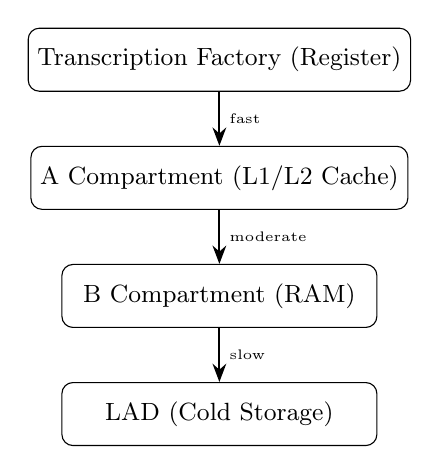
\begin{tikzpicture}[
  every node/.style={draw, rounded corners, minimum width=4cm, minimum height=0.8cm, align=center, font=\small},
  level/.style={-{Stealth}, thick}
]
\node (reg) at (0, 4.5) {Transcription Factory (Register)};
\node (l1) at (0, 3) {A Compartment (L1/L2 Cache)};
\node (ram) at (0, 1.5) {B Compartment (RAM)};
\node (disk) at (0, 0) {LAD (Cold Storage)};

\draw[level] (reg) -- (l1) node[midway, right, draw=none, minimum width=0pt] {\tiny fast};
\draw[level] (l1) -- (ram) node[midway, right, draw=none, minimum width=0pt] {\tiny moderate};
\draw[level] (ram) -- (disk) node[midway, right, draw=none, minimum width=0pt] {\tiny slow};
\end{tikzpicture}
\end{center}

\subsection{Radial Position and Access Latency}

The radial position of a genomic locus within the nucleus correlates with its transcriptional activity. Gene-rich chromosomes tend to occupy central positions, while gene-poor chromosomes are peripheral. This radial organization creates a continuous gradient of accessibility:

\begin{definition}[Radial Access Function]\label{def:radial-access}
The radial access function maps nuclear position to access latency:
\[
  \texttt{radial\_latency}(r) = \lambda_0 + \lambda_1 \cdot \left(\frac{r}{R_{\text{nucleus}}}\right)^\gamma
\]
where $r$ is the radial distance from the nuclear center, $R_{\text{nucleus}}$ is the nuclear radius, $\lambda_0$ is the base latency, $\lambda_1$ is the peripheral penalty, and $\gamma > 0$ controls the steepness of the gradient.
\end{definition}

This function captures the observation that loci near the nuclear periphery (large $r$) have higher access latency (lower transcriptional activity) than loci near the center (small $r$). The exponent $\gamma$ can be calibrated from experimental data relating nuclear position to gene expression levels.


%% ============================================================
%%  SECTION 8: FORMAL PROPERTIES
%% ============================================================
\section{Formal Properties}\label{sec:formal}

We now state and prove the three central theorems of our framework. These theorems establish that the type-theoretic model faithfully captures the essential properties of genome structural organization.

\subsection{Telomere Linear Type Theorem}

\begin{theorem}[Telomere Resource Soundness]\label{thm:telomere}
Let $S_0$ be a well-formed structure with $S_0.\texttt{telomeres}(c) = \texttt{Telomere}(n)$ for chromosome $c$. Let $S_0 \xrightarrow{\texttt{divide}} S_1 \xrightarrow{\texttt{divide}} \cdots \xrightarrow{\texttt{divide}} S_k$ be a sequence of $k$ division steps without telomerase activity. Then:
\begin{enumerate}[label=(\alph*)]
  \item $S_i.\texttt{telomeres}(c) = \texttt{Telomere}(n - i)$ for all $0 \leq i \leq k$.
  \item The sequence is well-typed only if $k \leq n$.
  \item If $k = n$, then $S_n.\texttt{telomeres}(c) = \texttt{Telomere}(0)$ and no further division is possible.
\end{enumerate}
\end{theorem}

\begin{proof}
We proceed by induction on $k$.

\textbf{Base case} ($k = 0$): The structure $S_0$ has $\texttt{Telomere}(n)$, and no divisions have occurred. Part (a) holds trivially with $S_0.\texttt{telomeres}(c) = \texttt{Telomere}(n - 0) = \texttt{Telomere}(n)$.

\textbf{Inductive step}: Assume the theorem holds for $k = m$, so $S_m.\texttt{telomeres}(c) = \texttt{Telomere}(n - m)$. Consider the $(m+1)$-th division. By the typing rule (\textsc{T-Divide}):
\[
  \texttt{divide} : \texttt{Telomere}(n - m) \multimap \texttt{Telomere}(n - m - 1) \otimes \texttt{DaughterCell}
\]
This rule is well-typed only if $n - m \geq 1$, i.e., $m + 1 \leq n$, i.e., $k \leq n$. After the division:
\[
  S_{m+1}.\texttt{telomeres}(c) = \texttt{Telomere}(n - (m+1))
\]
which establishes part (a) for $k = m + 1$.

For part (b), the typing rule (\textsc{T-Divide}) requires its input to have type $\texttt{Telomere}(j+1)$ for some $j \geq 0$. At step $i$, the input has type $\texttt{Telomere}(n - i + 1)$, which requires $n - i + 1 \geq 1$, i.e., $i \leq n$. Therefore $k \leq n$.

For part (c), if $k = n$, then $S_n.\texttt{telomeres}(c) = \texttt{Telomere}(0)$. The only well-typed operation on $\texttt{Telomere}(0)$ is $\texttt{senesce}$ (by \cref{def:senescence}). The rule (\textsc{T-Divide}) is not applicable since it requires $\texttt{Telomere}(j+1)$ and $\texttt{Telomere}(0)$ cannot be decomposed as $\texttt{Telomere}(j+1)$ for any $j \in \mathbb{N}$.

By linearity, the telomere resource at each step is consumed exactly once (no duplication or discarding), which ensures that the count decreases monotonically by exactly 1 per division. This completes the proof.
\end{proof}

\subsection{TAD Encapsulation Theorem}

\begin{theorem}[TAD Encapsulation]\label{thm:tad-encapsulation}
Let $T_1 = \texttt{TAD}(a_1, b_1, \beta_L^1, \beta_R^1)$ and $T_2 = \texttt{TAD}(a_2, b_2, \beta_L^2, \beta_R^2)$ be non-overlapping, non-nested TADs with all intervening boundaries having insulation score 1. Then for any well-formed structure $S$:
\begin{enumerate}[label=(\alph*)]
  \item No regulatory interaction originating in $T_1$ can reach a target in $T_2$.
  \item The contact frequency between any locus $x \in T_1$ and $y \in T_2$ satisfies $M_{xy} \leq \tau_{\text{inter}}$.
  \item Disruption of a boundary (reducing its insulation score below 1) is necessary and sufficient for cross-domain interaction.
\end{enumerate}
\end{theorem}

\begin{proof}
\textbf{Part (a):} By \cref{def:tad-access}, the access permission for $x \in T_1$ and $y \in T_2$ is:
\[
  \texttt{access}(x, y) = \prod_{b \in \texttt{Boundaries}(x,y)} (1 - b.\texttt{insulation\_score})
\]
Since $T_1$ and $T_2$ are non-overlapping and non-nested, there exists at least one boundary $b^*$ between them. By hypothesis, $b^*.\texttt{insulation\_score} = 1$, so:
\[
  \texttt{access}(x, y) \leq (1 - 1) = 0
\]
Since $\texttt{access}(x,y) = 0 < \theta$ for any positive threshold $\theta$, no regulatory interaction from $T_1$ can reach $T_2$.

\textbf{Part (b):} By the well-formedness condition (WF1) in \cref{def:well-formed}, loci in different TADs separated by a strong boundary (insulation score 1) satisfy $M_{xy} \leq \tau_{\text{inter}}$. Since all intervening boundaries have insulation score 1, this condition applies.

\textbf{Part (c):} \emph{Necessity}: If all boundaries retain insulation score 1, then by part (a), $\texttt{access}(x,y) = 0$ and no cross-domain interaction is possible. Therefore, boundary disruption is necessary.

\emph{Sufficiency}: Suppose a single boundary $b^*$ has its insulation score reduced to $s < 1$. If all other boundaries between $T_1$ and $T_2$ also have scores less than 1 (or $b^*$ is the only intervening boundary), then:
\[
  \texttt{access}(x, y) = \prod_{b} (1 - b.\texttt{insulation\_score}) > 0
\]
For sufficiently small threshold $\theta$, $\texttt{access}(x,y) > \theta$, and cross-domain interaction becomes possible. In the minimal case where $b^*$ is the sole intervening boundary, $\texttt{access}(x,y) = 1 - s > 0$, which exceeds $\theta$ for $\theta < 1 - s$.
\end{proof}

\subsection{Territory Memory Protection Theorem}

\begin{theorem}[Territory Memory Protection]\label{thm:territory}
Let $T_c = \texttt{Territory}(c)$ be the chromosome territory for chromosome $c$, and let the nuclear organization define a partition of the genome into territories. Then:
\begin{enumerate}[label=(\alph*)]
  \item \textbf{Isolation}: For chromosomes $c_1 \neq c_2$ and loci $x \in T_{c_1}$, $y \in T_{c_2}$, the interaction frequency satisfies:
  \[
    M_{xy} \leq \epsilon_{\text{inter-territory}}
  \]
  where $\epsilon_{\text{inter-territory}} \ll \tau_{\text{intra-territory}}$.
  \item \textbf{Self-containment}: For any chromosome $c$, the fraction of interactions involving loci outside $T_c$ is bounded:
  \[
    \frac{\sum_{y \notin T_c} M_{xy}}{\sum_{y} M_{xy}} \leq \delta \quad \text{for all } x \in T_c
  \]
  where $\delta \ll 1$ (typically $\delta \approx 0.1$ in Hi-C data).
  \item \textbf{Access hierarchy}: Access from $x$ to $y$ traverses the memory hierarchy:
  \[
    \texttt{latency}(x, y) = \texttt{base\_latency} + \sum_{L \in \texttt{levels}(x,y)} \texttt{penalty}(L)
  \]
  where $\texttt{levels}(x,y)$ is the set of hierarchy levels that must be crossed.
\end{enumerate}
\end{theorem}

\begin{proof}
\textbf{Part (a):} By \cref{def:territory}, chromosome territories occupy distinct nuclear regions with bounded overlap. The contact frequency between loci in different territories is limited by the physical distance between territories. Let $d(T_{c_1}, T_{c_2})$ be the nuclear distance between territories. By the polymer physics of chromatin, contact frequency decays as a power law:
\[
  M_{xy} \leq \frac{C}{d(x,y)^\gamma} \leq \frac{C}{d(T_{c_1}, T_{c_2})^\gamma} \coloneqq \epsilon_{\text{inter-territory}}
\]
where $\gamma \approx 1$ for interchromosomal contacts. Since territory centers are separated by distances much larger than the typical intra-territory distance, $\epsilon_{\text{inter-territory}} \ll \tau_{\text{intra-territory}}$.

\textbf{Part (b):} This follows from part (a) by summation. The inter-territory contacts are each bounded by $\epsilon_{\text{inter-territory}}$, while intra-territory contacts are at least $\tau_{\text{intra-territory}}$. Since the number of intra-territory loci scales as $L_c$ (chromosome length) and the total genomic size is $\sum_c L_c$, the ratio of inter- to total contacts for any locus $x \in T_c$ is:
\[
  \frac{\sum_{y \notin T_c} M_{xy}}{\sum_y M_{xy}} \leq \frac{(\sum_{c' \neq c} L_{c'}) \cdot \epsilon_{\text{inter-territory}}}{L_c \cdot \tau_{\text{intra-territory}} + (\sum_{c' \neq c} L_{c'}) \cdot \epsilon_{\text{inter-territory}}}
\]
Since $\epsilon_{\text{inter-territory}} \ll \tau_{\text{intra-territory}}$, this ratio is bounded by a small constant $\delta$.

\textbf{Part (c):} Define the hierarchy levels as:
\begin{itemize}
  \item $L_0$: Same sub-TAD (base latency only).
  \item $L_1$: Same TAD, different sub-TADs (one boundary crossing).
  \item $L_2$: Same territory, different TADs (TAD boundary penalty).
  \item $L_3$: Different territories (inter-territory penalty).
\end{itemize}
The penalty is additive because each level crossing introduces an independent physical barrier. The set $\texttt{levels}(x,y)$ is determined by the lowest common ancestor of $x$ and $y$ in the hierarchy tree. If $x$ and $y$ share a sub-TAD, $\texttt{levels}(x,y) = \emptyset$ and latency is minimal. If they are in different territories, $\texttt{levels}(x,y) = \{L_1, L_2, L_3\}$ and latency is maximal. This establishes the claimed access hierarchy.
\end{proof}

\subsection{Additional Formal Results}

\begin{proposition}[Loop-TAD Compatibility]\label{prop:loop-tad}
Let $\ell = \texttt{ChromatinLoop}(\alpha, \beta)$ be a chromatin loop in a well-formed structure. If both anchors lie within the same TAD $T$, then dereferencing $\ell$ does not violate TAD encapsulation. If the anchors lie in different TADs $T_1, T_2$, then dereferencing requires $\texttt{access}(\alpha, \beta) > \theta$.
\end{proposition}

\begin{proof}
If both anchors are in the same TAD, the loop is an intra-TAD contact, which is permitted by the well-formedness conditions (WF1 does not restrict intra-TAD contacts). If the anchors are in different TADs, dereferencing requires physical contact between the anchors. By \cref{def:deref}, condition (i) requires that both anchors be in the same TAD or that the intervening boundaries be permeable. The latter condition is precisely $\texttt{access}(\alpha, \beta) > \theta$ from \cref{def:tad-access}.
\end{proof}

\begin{corollary}[Structural Variant Pathology]\label{cor:sv-pathology}
A structural variant that repositions a TAD boundary (e.g., a deletion removing a CTCF site) can create novel cross-domain loops, potentially activating oncogenes through ectopic enhancer-promoter contacts.
\end{corollary}

\begin{proof}
By \cref{thm:tad-encapsulation}, part (c), removing a boundary (reducing insulation score to 0) is sufficient to enable cross-domain interactions. If an enhancer in $T_1$ and an oncogene promoter in $T_2$ are now accessible, the cohesin pointer manager (\cref{def:cohesin-manager}) can form a novel loop $\texttt{ChromatinLoop}(\texttt{Enhancer}, \texttt{Promoter})$. Dereferencing this loop produces a $\texttt{TranscriptionEvent}$ activating the oncogene. This mechanism has been experimentally validated in cases such as the \emph{EPHA3} activation by TAD boundary disruption in T-cell acute lymphoblastic leukemia.
\end{proof}

\begin{lemma}[Compartment Transition Preserves Well-Formedness]\label{lem:compartment}
The compartment transition operations $\texttt{activate}$ and $\texttt{silence}$ preserve the well-formedness of the memory hierarchy. Specifically, if $S$ is well-formed and $S'$ is obtained by transitioning locus $x$ from compartment B to compartment A, then $S'$ is well-formed provided $\texttt{accessibility}(x)$ is updated to satisfy $\texttt{accessibility}(x) \geq 0.5$.
\end{lemma}

\begin{proof}
The well-formedness condition (WF2) requires compartment A loci to have accessibility $\geq 0.5$ and compartment B loci to have accessibility $< 0.5$. Transitioning $x$ from B to A and simultaneously updating $\texttt{accessibility}(x) \geq 0.5$ preserves (WF2) for $x$. All other loci are unchanged, so their conditions are preserved. Conditions (WF1), (WF3), and (WF4) are independent of the compartment assignment of a single locus (TAD structure, territories, and telomeres are unchanged), so they are trivially preserved.
\end{proof}

\begin{proposition}[Telomerase Extension Commutes with Non-Division Morphisms]\label{prop:telomerase-commute}
Let $f : \texttt{Structure}\langle G_1 \rangle \to \texttt{Structure}\langle G_2 \rangle$ be a structure morphism that does not alter telomere state (a non-division morphism, e.g., compartment switching). Then for any chromosome $c$:
\[
  f \circ \texttt{extend}_c = \texttt{extend}_c \circ f
\]
That is, telomerase extension commutes with non-division morphisms.
\end{proposition}

\begin{proof}
Since $f$ does not alter telomere state, $f(S).\texttt{telomeres}(c) = S.\texttt{telomeres}(c)$ for all $c$. The $\texttt{extend}_c$ operation modifies only the telomere field for chromosome $c$, while $f$ modifies only non-telomere fields (accessibility, compartment assignments, loop configurations, etc.). Since the two operations act on disjoint fields of the structure record, they commute:
\[
  (f \circ \texttt{extend}_c)(S).\texttt{telomeres}(c) = f(\texttt{extend}_c(S)).\texttt{telomeres}(c) = \texttt{Telomere}(n + k)
\]
\[
  (\texttt{extend}_c \circ f)(S).\texttt{telomeres}(c) = \texttt{extend}_c(f(S)).\texttt{telomeres}(c) = \texttt{Telomere}(n + k)
\]
and all non-telomere fields are identical in both compositions.
\end{proof}


%% ============================================================
%%  SECTION 9: HASKELL IMPLEMENTATION
%% ============================================================
\section{Haskell Implementation}\label{sec:haskell}

We provide a Haskell implementation that captures the core types and operations of our framework. The implementation uses Haskell's type system to enforce linearity constraints (via GADTs and DataKinds) and to model the structural hierarchy.

\begin{lstlisting}[language=DNALang, caption={Core types for the structural DNA memory architecture}]
{-# LANGUAGE GADTs, DataKinds, KindSignatures, TypeFamilies #-}

module StructuralDNA where

import Data.Kind (Type)

-- Natural numbers at the type level
data Nat = Z | S Nat

-- Telomere as a linear resource indexed by repeat count
data Telomere (n :: Nat) where
  TelomereZ :: Telomere Z
  TelomereS :: Telomere n -> Telomere (S n)

-- Division consumes one telomeric repeat
divide :: Telomere (S n) -> (Telomere n, DaughterCell)
divide (TelomereS t) = (t, DaughterCell)

-- Senescence for zero-length telomeres
senesce :: Telomere Z -> SenescentCell
senesce TelomereZ = SenescentCell

-- Telomerase extends telomeric repeats
extend :: Telomere n -> TelomeraseAccess -> Telomere (S n)
extend t _ = TelomereS t

data DaughterCell = DaughterCell deriving Show
data SenescentCell = SenescentCell deriving Show
data TelomeraseAccess = GermCell | StemCell
\end{lstlisting}

\begin{lstlisting}[language=DNALang, caption={TAD and boundary types}]
-- CTCF orientation
data CTCFOrientation = Forward | Reverse
  deriving (Eq, Show)

-- Boundary with insulation score
data Boundary = Boundary
  { ctcfOrientation :: CTCFOrientation
  , cohesinLoaded   :: Bool
  , insulationScore :: Double  -- in [0,1]
  } deriving Show

-- TAD as a memory segment with boundaries
data TAD = TAD
  { tadStart    :: Int
  , tadEnd      :: Int
  , leftBound   :: Boundary
  , rightBound  :: Boundary
  } deriving Show

-- Check well-formedness: convergent CTCF
isWellFormed :: TAD -> Bool
isWellFormed tad =
  ctcfOrientation (leftBound tad) == Forward &&
  ctcfOrientation (rightBound tad) == Reverse

-- Access control between loci in different TADs
accessPermission :: [Boundary] -> Double
accessPermission = product . map (\b -> 1.0 - insulationScore b)

-- Check if access is granted
canAccess :: [Boundary] -> Double -> Bool
canAccess boundaries threshold =
  accessPermission boundaries > threshold
\end{lstlisting}

\begin{lstlisting}[language=DNALang, caption={Chromatin loops as typed pointers}]
-- Locus types at the value level
data LocusType = Enhancer | Promoter | CTCFSite | Other
  deriving (Eq, Show)

-- Genomic locus
data GenomicLocus = GenomicLocus
  { chromosome :: Int
  , position   :: Int
  , locusType  :: LocusType
  } deriving Show

-- Chromatin loop as a pointer between loci
data ChromatinLoop = ChromatinLoop
  { anchorSource :: GenomicLocus
  , anchorTarget :: GenomicLocus
  , loopStrength :: Double
  } deriving Show

-- Dereference: enhancer-promoter activation
data TranscriptionEvent = TranscriptionEvent
  { targetGene :: GenomicLocus
  , txnLevel   :: Double
  } deriving Show

deref :: ChromatinLoop -> Double -> Maybe TranscriptionEvent
deref loop accessThreshold
  | locusType (anchorSource loop) == Enhancer
  , locusType (anchorTarget loop) == Promoter
  , loopStrength loop > accessThreshold
  = Just (TranscriptionEvent (anchorTarget loop)
                             (loopStrength loop))
  | otherwise = Nothing
\end{lstlisting}

\begin{lstlisting}[language=DNALang, caption={Nuclear memory hierarchy}]
-- Compartment assignment
data Compartment = CompartmentA | CompartmentB
  deriving (Eq, Show)

-- Memory hierarchy levels
data MemoryLevel
  = Register       -- transcription factory
  | L1Cache        -- A compartment, euchromatin
  | MainMemory     -- B compartment, heterochromatin
  | ColdStorage    -- lamina-associated domain
  deriving (Eq, Ord, Show)

-- Territory as a memory bank
data Territory = Territory
  { territoryChrom  :: Int
  , nuclearPosition :: (Double, Double, Double)
  , territoryVolume :: Double
  } deriving Show

-- Access latency computation
accessLatency :: MemoryLevel -> MemoryLevel -> Double
accessLatency src dst = abs (cost dst - cost src)
  where
    cost Register    = 1.0
    cost L1Cache     = 5.0
    cost MainMemory  = 20.0
    cost ColdStorage = 100.0

-- The full Structure type
data Structure = Structure
  { structTADs          :: [TAD]
  , structLoops         :: [ChromatinLoop]
  , structTerritories   :: [Territory]
  , structCompartments  :: GenomicLocus -> Compartment
  , structAccessibility :: GenomicLocus -> Double
  }
\end{lstlisting}


%% ============================================================
%%  SECTION 10: DISCUSSION AND CONCLUSION
%% ============================================================
\section{Discussion and Conclusion}\label{sec:discussion}

\subsection{Summary of Contributions}

We have presented a type-theoretic framework that formalizes the structural elements of the genome as components of a memory architecture. The key mappings are:

\begin{itemize}
  \item \textbf{Telomeres} $\longleftrightarrow$ \textbf{Linear resources}: The progressive shortening of telomeres with each cell division is captured by a linear type system where each division consumes one unit of a finite resource. The Hayflick limit emerges as a type-level constraint.
  \item \textbf{Centromeres} $\longleftrightarrow$ \textbf{Synchronization primitives}: The spindle assembly checkpoint is a barrier that requires all chromosomes to report attachment before anaphase proceeds. Kinetochore singularity is enforced by mutual exclusion.
  \item \textbf{TADs} $\longleftrightarrow$ \textbf{Memory segments}: TAD boundaries enforced by convergent CTCF and cohesin provide insulation analogous to memory segment protection, with quantitative insulation scores governing cross-boundary access.
  \item \textbf{Chromatin loops} $\longleftrightarrow$ \textbf{Typed pointers}: Enhancer-promoter loops are pointers that, when dereferenced, activate transcription. Cohesin manages the pointer lifecycle through extrusion, stalling, and release.
  \item \textbf{Nuclear organization} $\longleftrightarrow$ \textbf{Memory hierarchy}: Chromosome territories, A/B compartments, and LADs map onto a multi-level memory hierarchy with increasing access latency.
\end{itemize}

\subsection{Biological Implications}

The framework provides a unified computational lens for understanding several biological phenomena:

\begin{enumerate}[label=(\roman*)]
  \item \textbf{Aging}: Telomere attrition is resource exhaustion. The Hayflick limit is a compile-time (type-level) guarantee that replicative capacity is finite.
  \item \textbf{Cancer}: Telomerase reactivation is a capability violation; TAD boundary disruption creates dangling pointers and ectopic enhancer-promoter contacts. Both are ``type errors'' in the genome's structural program.
  \item \textbf{Development}: Cell differentiation involves large-scale reorganization of the memory hierarchy---compartment switching, LAD repositioning, and loop rewiring---corresponding to a complete memory remapping.
  \item \textbf{Structural variants}: Deletions, inversions, and translocations that disrupt TAD boundaries or loop anchors are pointer corruption events with predictable pathological consequences.
\end{enumerate}

\subsection{Connections to Programming Language Design}

Our framework suggests that programming language design can draw inspiration from genome organization. The genome's use of linear types for resource management, barriers for synchronization, segments for isolation, and pointers for long-range communication represents a system that has been refined by billions of years of evolution. Specific insights include:

\begin{itemize}
  \item \textbf{Bounded linear types}: The telomere model suggests that parameterizing linear types by a resource count enables fine-grained tracking of resource lifetimes, going beyond the binary used/unused distinction of standard linear types.
  \item \textbf{Insulation scores}: The quantitative insulation model for TAD boundaries suggests that access control need not be binary; graded permissions parameterized by a real-valued score could model partial isolation in concurrent systems.
  \item \textbf{Hierarchical memory}: The nuclear memory hierarchy suggests that programming languages could benefit from explicit memory hierarchy annotations, allowing programmers to reason about data placement and access patterns.
\end{itemize}

\subsection{Limitations and Future Work}

Several aspects of genome structure are not yet captured by our framework:

\begin{itemize}
  \item \textbf{Dynamics}: Our model is largely static; a process-algebraic extension could capture the dynamic aspects of loop extrusion and compartment switching.
  \item \textbf{Stochasticity}: Genome organization is inherently stochastic at the single-cell level. Incorporating probabilistic types or measure-theoretic semantics is a natural extension.
  \item \textbf{Phase separation}: Recent work suggests that many nuclear compartments are formed by liquid-liquid phase separation, which introduces a physical mechanism not yet captured by our type-theoretic model.
  \item \textbf{Replication}: The interplay between replication timing and the memory hierarchy deserves formal treatment.
  \item \textbf{Epigenetic marks}: Histone modifications and DNA methylation affect chromatin accessibility and should be integrated as annotations on the memory hierarchy.
\end{itemize}

\subsection{Conclusion}

By treating structural DNA elements as components of a memory architecture, we gain a precise, formal language for reasoning about genome organization. The type-theoretic framework enables us to state and prove properties---resource soundness for telomeres, encapsulation for TADs, protection for territories---that have direct biological interpretations. The Haskell implementation demonstrates that these formal constructs yield executable specifications, bridging the gap between mathematical biology and computational practice.

The genome is not just a program; it is an entire computing system, complete with memory management, access control, synchronization, and hierarchical storage. Understanding its architecture through the lens of programming language theory opens new avenues for both computational biology and programming language design.

\subsection*{Acknowledgments}

The author thanks the members of the YonedaAI Collaboration for valuable discussions on category theory, type theory, and their applications to biological systems.

\begin{thebibliography}{99}

\bibitem{lieberman2009comprehensive}
E.~Lieberman-Aiden, N.~L.~van Berkum, L.~Williams, et al.,
``Comprehensive mapping of long-range interactions reveals folding principles of the human genome,''
\textit{Science}, vol.~326, no.~5950, pp.~289--293, 2009.

\bibitem{dixon2012topological}
J.~R.~Dixon, S.~Selvaraj, F.~Yue, et al.,
``Topological domains in mammalian genomes identified by analysis of chromatin interactions,''
\textit{Nature}, vol.~485, no.~7398, pp.~376--380, 2012.

\bibitem{rao20143d}
S.~S.~P.~Rao, M.~H.~Huntley, N.~C.~Durand, et al.,
``A 3D map of the human genome at kilobase resolution reveals principles of chromatin looping,''
\textit{Cell}, vol.~159, no.~7, pp.~1665--1680, 2014.

\bibitem{blackburn2001telomere}
E.~H.~Blackburn,
``Switching and signaling at the telomere,''
\textit{Cell}, vol.~106, no.~6, pp.~661--673, 2001.

\bibitem{olovnikov1973theory}
A.~M.~Olovnikov,
``A theory of marginotomy: the incomplete copying of template margin in enzymic synthesis of polynucleotides and biological significance of the phenomenon,''
\textit{Journal of Theoretical Biology}, vol.~41, no.~1, pp.~181--190, 1973.

\bibitem{hayflick1961serial}
L.~Hayflick and P.~S.~Moorhead,
``The serial cultivation of human diploid cell strains,''
\textit{Experimental Cell Research}, vol.~25, no.~3, pp.~585--621, 1961.

\bibitem{girard1987linear}
J.-Y.~Girard,
``Linear logic,''
\textit{Theoretical Computer Science}, vol.~50, no.~1, pp.~1--101, 1987.

\bibitem{wadler1990linear}
P.~Wadler,
``Linear types can change the world!''
in \textit{Programming Concepts and Methods}, 1990.

\bibitem{bray1995protein}
D.~Bray,
``Protein molecules as computational elements in living cells,''
\textit{Nature}, vol.~376, no.~6538, pp.~307--312, 1995.

\bibitem{regev2001representation}
A.~Regev and E.~Shapiro,
``Cellular abstractions: cells as computation,''
\textit{Nature}, vol.~419, no.~6905, p.~343, 2001.

\bibitem{cardelli2005abstract}
L.~Cardelli,
``Abstract machines of systems biology,''
\textit{Transactions on Computational Systems Biology III}, pp.~145--168, 2005.

\bibitem{encode2012integrated}
The ENCODE Project Consortium,
``An integrated encyclopedia of DNA elements in the human genome,''
\textit{Nature}, vol.~489, no.~7414, pp.~57--74, 2012.

\bibitem{dekker2013exploring}
J.~Dekker, A.~Marti-Renom, and L.~A.~Mirny,
``Exploring the three-dimensional organization of genomes: interpreting chromatin interaction data,''
\textit{Nature Reviews Genetics}, vol.~14, no.~6, pp.~390--403, 2013.

\bibitem{nora2012spatial}
E.~P.~Nora, B.~R.~Lajoie, E.~G.~Schulz, et al.,
``Spatial partitioning of the regulatory landscape of the X-inactivation centre,''
\textit{Nature}, vol.~485, no.~7398, pp.~381--385, 2012.

\bibitem{fudenberg2016formation}
G.~Fudenberg, M.~Imakaev, C.~Lu, et al.,
``Formation of chromosomal domains by loop extrusion,''
\textit{Cell Reports}, vol.~15, no.~9, pp.~2038--2049, 2016.

\bibitem{sanborn2015chromatin}
A.~L.~Sanborn, S.~S.~P.~Rao, S.-C.~Huang, et al.,
``Chromatin extrusion explains key features of loop and domain formation in wild-type and engineered genomes,''
\textit{Proceedings of the National Academy of Sciences}, vol.~112, no.~47, pp.~E6456--E6465, 2015.

\bibitem{fullwood2009oestrogen}
M.~J.~Fullwood, M.~H.~Liu, Y.~F.~Pan, et al.,
``An oestrogen-receptor-$\alpha$-bound human chromatin interactome,''
\textit{Nature}, vol.~462, no.~7269, pp.~58--64, 2009.

\bibitem{cremer2001chromosome}
T.~Cremer and C.~Cremer,
``Chromosome territories, nuclear architecture and gene regulation in mammalian cells,''
\textit{Nature Reviews Genetics}, vol.~2, no.~4, pp.~292--301, 2001.

\bibitem{guelen2008domain}
L.~Guelen, L.~Pagie, E.~Brasset, et al.,
``Domain organization of human chromosomes revealed by mapping of nuclear lamina interactions,''
\textit{Nature}, vol.~453, no.~7197, pp.~948--951, 2008.

\end{thebibliography}

\end{document}
